\documentclass[border=4pt]{standalone}
\usepackage{tikz}
\usetikzlibrary{arrows.meta}
\begin{document}
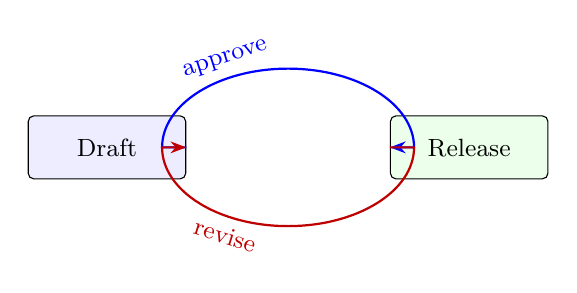
\begin{tikzpicture}[
  auto,
  state/.style={draw,rounded corners=2pt,minimum width=20mm,minimum height=8mm,fill=blue!7},
  flow/.style={-{Stealth[length=2mm]},thick},
  every node/.append style={font=\small}
]
  \node[state] (draft) at (-2.3,0) {Draft};
  \node[state,fill=green!8] (release) at (2.3,0) {Release};

  \draw[flow,blue] (draft.east) -- (-1.6,0)
    arc[start angle=180,end angle=0,x radius=1.6cm,y radius=1cm]
    node[pos=.35,sloped] {approve} -- (release.west);
  \draw[flow,red!75!black] (release.west) -- (1.6,0)
    arc[start angle=0,end angle=-180,x radius=1.6cm,y radius=1cm]
    node[pos=.65,sloped,swap] {revise} -- (draft.east);
\end{tikzpicture}
\end{document}
